\documentclass[11pt,a4paper]{article}
\usepackage[utf8]{inputenc}
\usepackage[activeacute,spanish]{babel}
\usepackage{graphicx}
\author{Miguel Angel Aguirre Olvera}
\title{Tarea 4 compiladores e interpretes}
\usepackage{multicol}
\DeclareGraphicsExtensions{.jpg}

\begin{document}
\maketitle
\begin{multicols}{2}
\begin{center}
\textbf{Compilador}
\end{center}
Es un programa informatico que traduce un programa escrito en un lenguaje de programacion a otro lenguaje de programacion, generando un programa equivalente que la maquina sera capaz de interpretar 
Un compilador es un programa que permite traducir el codigo fuente de un programa en lenguaje de alto nivel a otro de leguaje inferior (lenguaje maquina) de esta manera un programador puede diseñar un programa en un lenguaje mas cercano a como piensa un humano para luego compilarlo a un programa mas manejable por la maquina 
\begin{center}
\textbf{Interprete}
\end{center}
Es un programa informatico capaz de analizar y ejecutar otros programas escritos en un lenguaje de alto nivel. Los interpretes se diferencian de los compiladores en que mientras estos producen un programa desde su descripcion en un lenguaje de programacion o codigo maquina del sistema, los intérpretes sólo realizan la traducción a medida que sea necesaria, típicamente, instrucción por instrucción, y normalmente no guardan el resultado de dicha traducción.Los programas interpretados suelen ser más lentos que los compilados debido a la necesidad de traducir el programa mientras se ejecuta, pero a cambio son más flexibles como entornos de programación y de puración (lo que se traduce, por ejemplo, en una mayor facilidad para reemplazar partes enteras del programa o añadir módulos completamente nuevos), y permiten ofrecer al programa interpretado un entorno no dependiente de la máquina donde se ejecuta el intérprete, sino del propio intérprete (lo que se conoce comúnmente como máquina virtual).
Usando un intérprete, un solo archivo fuente puede producir resultados iguales incluso en sistemas sumamente diferentes (ej. una PC y un PlayStation 3). Usando un compilador, un solo archivo fuente puede producir resultados iguales solo si es compilado a distintos ejecutables específicos a cada sistema.
\begin{center}
\textbf{Ejemplos}
\end{center}
\textbf{Compiladores}

c, c++, pascal, FORTRAN, cobol


\textbf{Interpretes}

BASIC QBASIC QUICKBASIC VISUALBASIC SMALTALK JAVA




\begin{center}
\textbf{librerias en C}
\end{center}
Es una recopilacion de ficheros, cabecera y bibliotecas con rutinas, estandarizadas por un comite ISO que implementan operaciones comunes tales como las de entrada y salida o el manejo de cadenas El nombre y las características de cada función, el prototipo, así como la definición de algunos tipos de datos y macros, se encuentran en un fichero denominado archivo de cabecera (con extensión ".h"), pero la implementación real de las funciones están separadas en un archivo de la biblioteca. La denominación y el ámbito de las cabeceras se han convertido en comunes, pero la organización de las bibliotecas sigue siendo diversa, ya que éstas suelen distribuirse con cada compilador. Dado que los compiladores de C, a menudo, ofrecen funcionalidades adicionales que no están especificados en el ANSI C, la biblioteca de un compilador no siempre es compatible con el estándar ni con las bibliotecas de otros compiladores.
\begin{center}
\textbf{Las mas usadas}
\end{center}

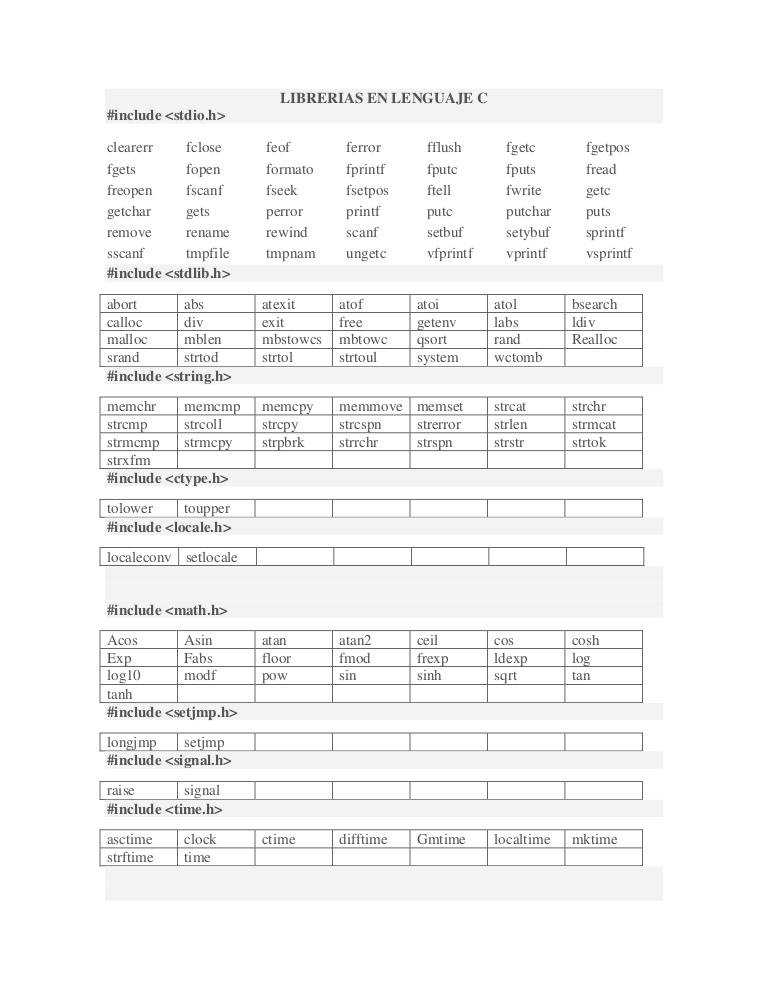
\includegraphics[scale=.40]{libreriac.jpg} 


\end{multicols}


\end{document}